\def \MOISEp {$\mathcal{M}OISE^+$ }

\chapter{Target System}
\label{ch:target_system}

To enable a better understanding of the proposed improvements, it is necessary to understand how the system worked before the changes. For this, the rules to which the system must obey and the organizational model used before the changes, following the structure of the \MOISEp model, will be explained, and, based on these two factors, the previous game strategy will be presented.

\section{Game Rules}
\label{sec:rules}

In this section, the relevant rules for understanding the game strategy will be presented, the complete rules of the category can be accessed at \cite{RulesVSSS}.

During a match, several events can happen that influence the game strategy used, the most important cases of the rules for the game strategy will be explained below. These events are sent to the team through the VSSReferee, which uses the UDP protocol to send messages.

The events received from the referee system can be divided into two types, the game events, and the control events. The game events are used to signalize something that happened in the game, for example, a foul, while the control events are used to indicate the flow of the game, for example, to signalize if the game is running or not.

The game events described in the rules are:

\begin{itemize}
    \item Free Kick: Event that occurs for specific types of fouls during the game, such as blocking the opponent's goalkeeper in his area, and which leads to a kick by the injured team from a certain marking on the field.
    \item Penalty: Event that covers different cases of fouls that are considered more serious, such as two robots inside the area actively defending the goal. This event leads to a kick by the injured team from the penalty spot, towards the opponent's goal. This event can also occur for game tiebreakers.
    \item Goal Kick: Event that occurs, in general, when there is a foul in the attack, such as if two attacking robots enter the opposing team's goal area, and which results in a kick by the injured team, which can position the ball in any position within their goal area.
    \item Free Ball: Event that occurs when there is a deadlock and the ball is stopped for more than five seconds outside the goal areas, which leads to a ball dispute, where the ball is positioned in the free ball marking of the quadrant in which it occurred.
    \item Kickoff: Event that occurs when the game is started or restarted due to the occurrence of a goal. When this event occurs, the ball is placed in the center of the field, so a new game can start. Depending on what happened in the event, one team will have repositioning priority over the other.
\end{itemize}

Meanwhile, the control events are specified as follows:

\begin{itemize}
    \item Game On: Event that indicates that the game is running.
    \item Stop: Event that indicates that the game is not running.
    \item Halt: Event that occurs when the game is halted so that a human referee can verify an occurrence in the game and take the necessary actions. Upon receiving this event, the team must be able to return to the exact state it was when it received the event flag.
\end{itemize}

\section{Organization Model}
\label{sec:organization_model}

Using the \MOISEp model, a mapping of the current solution was made, to validate the use of the model, facilitate the understanding of the current system and observe gaps for improvements. The structural specification of the team obtained from this mapping can be seen in Figure \ref{fig:moise_mapping}.

\begin{figure}[!ht]
    \centering
    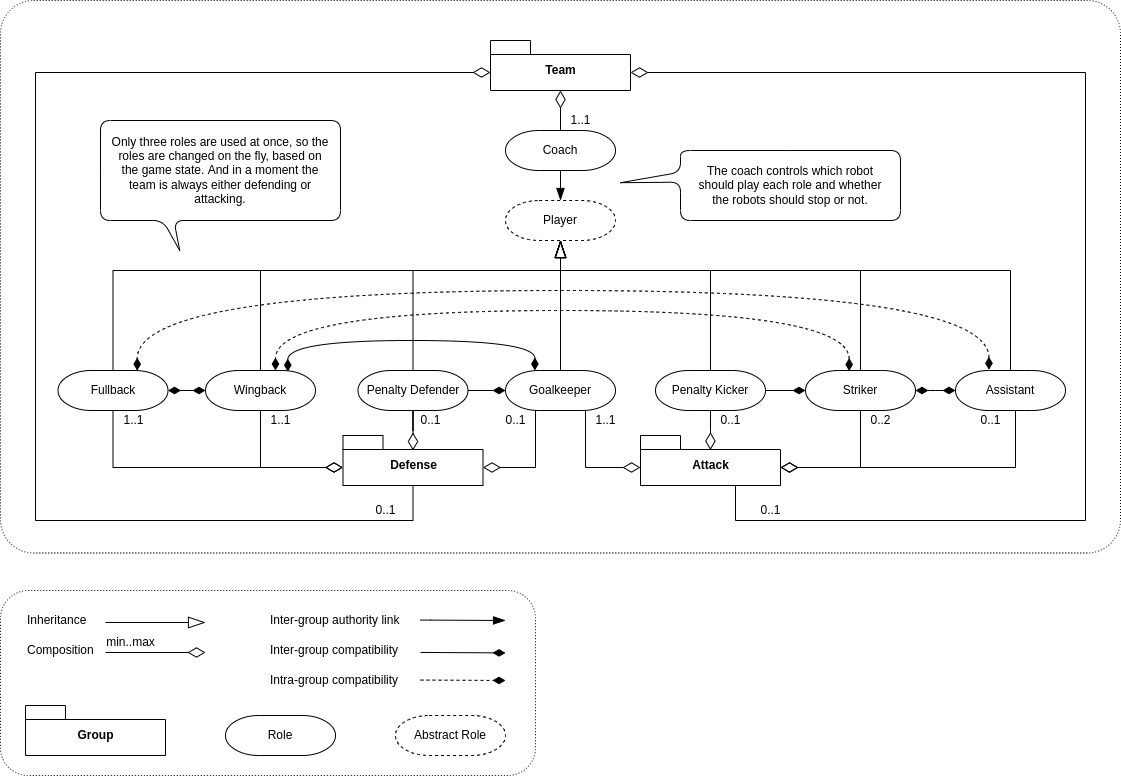
\includegraphics[width=\linewidth]{chapters/target_system/images/ThunderVolt Moise-Structural Specification.png}
    \caption{Mapping of the solution to the MOISE model made by the author}
    \label{fig:moise_mapping}
\end{figure}

A team of the VSSS category just plays using three robots, however, as it is possible to observe in the structural specification, to ensure greater versatility in what each robot can do, seven possible roles have been defined that the ThunderVolt's robots can play. These roles and their responsibilities are defined as follows:

\begin{itemize}
    \item Goalkeeper: Defends the goal.
    \item Striker: Carries out attacks against the opposing team.
    \item Assistant: Positions itself strategically to take advantage of rebounds in the attack.
    \item Penalty Kicker: Kicks penalties in the opposing team.
    \item Penalty Defender: Defends the opposing team's penalties.
    \item Fullback: Helps the goalkeeper to defend the goal
    \item Wingback: Helps the defense, while trying to make counterattacks.
\end{itemize}

It is important to note that the behaviors of these roles, meaning their functional specification, have already been implemented using behavior trees prior to this work. This experience of using behavior trees to define the roles to be performed proved to be quite advantageous, due to the ease of implementation, flexibility, and modularity. It is also noteworthy that in this organization the deontic specification is very straightforward since the roles present in the organization are actually differentiated according to their functional specification.

Regarding the listed roles, some of these are played while the team is attacking and others while the team is defending. As not all roles can be performed simultaneously, there is an agent in the organization, called Coach, which is responsible for assigning each of the three robots of the team a certain role in the game, being, therefore, the leader of the organization. Taking into account that a game is a dynamic scenario, as time progresses, it is also necessary to perform role swaps between the robots, these swaps are also coordinated by the Coach and depend on the role that each robot is playing at the moment.

Thus, for a robot that is playing a certain role to play another role, there must be a compatibility between the two roles, for example, the attacker role is not compatible with the goalkeeper role, due to different positioning and functionalities, meanwhile, the assistant and striker roles are compatible with each other, thanks to the high synergy between the two roles in the attack state.

In general, the roles of penalty kicker and defender are used only when a penalty event occurs, with the penalty kicker being used in place of the striker and the penalty defender in the place of the goalkeeper. However, the team supports many penalty modes, thus there is also the case where a penalty can be kicked by a striker or defended by the goalkeeper. In other moments of the game, while the team is defending, the roles of goalkeeper, fullback, and wingback are used, and while the team is attacking, the roles of goalkeeper, assistant, and striker are usually used instead. Besides that, in some special moments of the game, an extra striker can be used in place of the assistant to make the team more offensive.

To implement the Coach and all the swaps between the roles, the previous strategy used a finite state machine, which will be described in the next section.

\section{Game Strategy}

Bearing in mind the aforementioned roles and the compatibilities between them, which allows the swap of roles between the robots, a finite state machine was developed to define the game strategy, that is the behavior of the Coach agent. With the increasing complexity of the strategy, this solution proved to be non-scalable and not sustainable for the project, being a major gap for improvements in the previous system. The size of the strategy code significantly expanded, making it difficult for the FSM to accommodate and scale with the increased complexity.

\begin{figure}[!h]
    \centering
    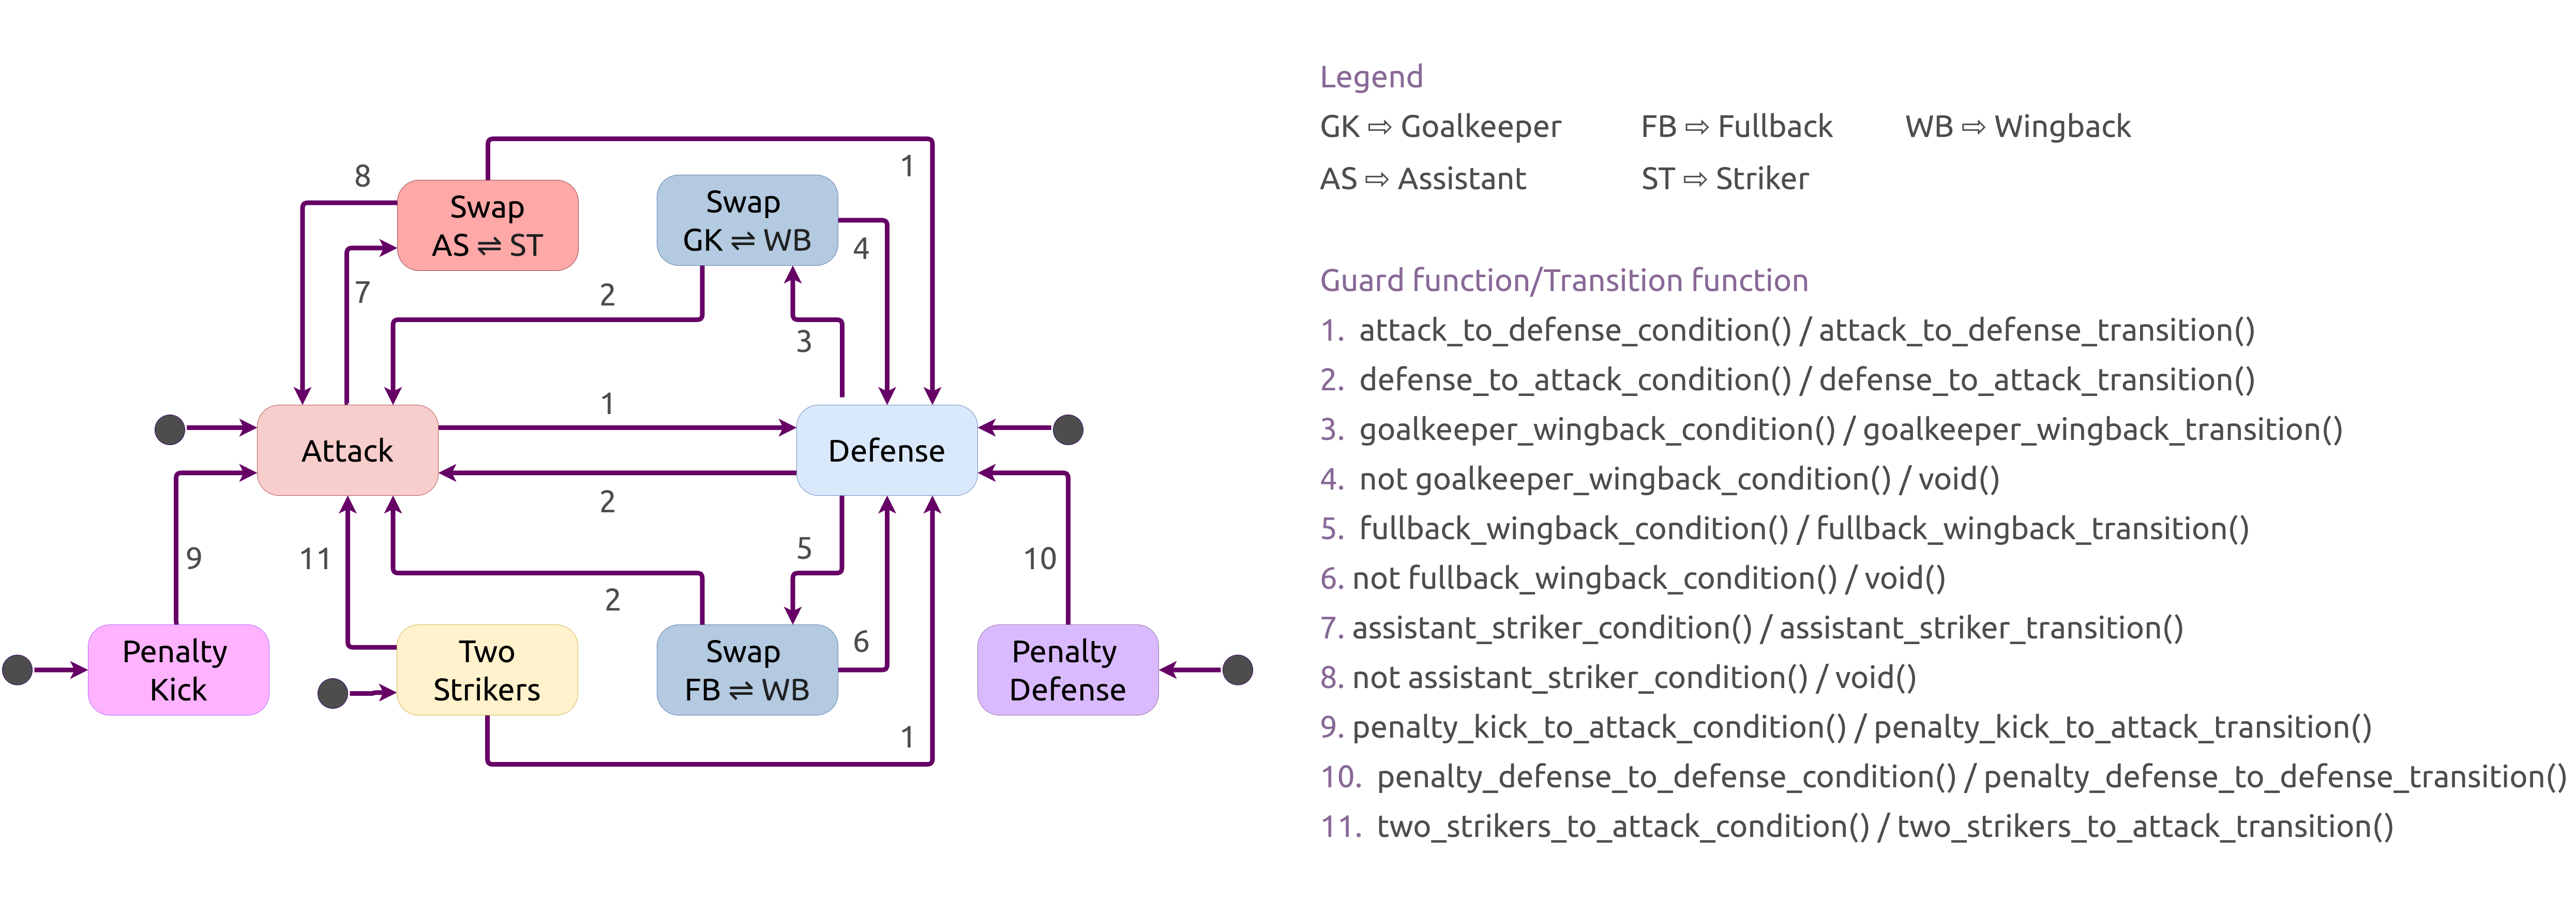
\includegraphics[width=\linewidth]{chapters/target_system/images/BehaviorsController FSM.png}
    \caption{Finite State Machine of game strategy diagram made by the author}
    \label{fig:behaviors_controller_fsm}
\end{figure}

The previous strategy can be seen in Figure \ref{fig:behaviors_controller_fsm}. In the FSM, there are eight possible states for the system. Among them, three are states where role swaps occur ("Swap AS $\rightleftharpoons$ ST", "Swap GK $\rightleftharpoons$ WB", and "Swap FB $\rightleftharpoons$ WB"), three are only entry states ("Penalty Kick", "Penalty Defense", and "Two Strikers"), and two are both entry and waiting states ("Attack" and "Defense"). The entry states define the initial roles configuration of the team, and the determination of which of the five possible entry states would be the state in which to start executing the FSM was made in advance upon receiving one of the events described in Section \ref{sec:rules}. For example, when a penalty event for the opposing team was received, the entry state was set to be the penalty defense state. Each transition between states was controlled by a guard function and when the condition of this function was satisfied, a transition function was called, all these functions are listed in Figure \ref{fig:behaviors_controller_fsm}. The guard functions were responsible for checking the conditions for changing roles, while transition functions handled the assignment of a new role to a robot according to the role it was performing and the compatibility of this role with other roles.

An important feature to note is that in all cases, to go to a swap state, a swap condition was analyzed, meanwhile, to exit these states and return to the attack or defense states, the negation of the swap condition was analyzed. This was necessary to ensure that the swap state was only exited when the swap was complete and could not happen immediately afterward, guaranteeing a hysteresis to the system and avoiding multiple subsequent swaps that would make the system unstable.
